\PassOptionsToPackage{unicode=true}{hyperref} % options for packages loaded elsewhere
\PassOptionsToPackage{hyphens}{url}
%
\documentclass[]{book}
\usepackage{lmodern}
\usepackage{amssymb,amsmath}
\usepackage{ifxetex,ifluatex}
\usepackage{fixltx2e} % provides \textsubscript
\ifnum 0\ifxetex 1\fi\ifluatex 1\fi=0 % if pdftex
  \usepackage[T1]{fontenc}
  \usepackage[utf8]{inputenc}
  \usepackage{textcomp} % provides euro and other symbols
\else % if luatex or xelatex
  \usepackage{unicode-math}
  \defaultfontfeatures{Ligatures=TeX,Scale=MatchLowercase}
\fi
% use upquote if available, for straight quotes in verbatim environments
\IfFileExists{upquote.sty}{\usepackage{upquote}}{}
% use microtype if available
\IfFileExists{microtype.sty}{%
\usepackage[]{microtype}
\UseMicrotypeSet[protrusion]{basicmath} % disable protrusion for tt fonts
}{}
\IfFileExists{parskip.sty}{%
\usepackage{parskip}
}{% else
\setlength{\parindent}{0pt}
\setlength{\parskip}{6pt plus 2pt minus 1pt}
}
\usepackage{hyperref}
\hypersetup{
            pdftitle={An Introduction to R},
            pdfauthor={Vittorio Perduca (Université de Paris)},
            pdfborder={0 0 0},
            breaklinks=true}
\urlstyle{same}  % don't use monospace font for urls
\usepackage{color}
\usepackage{fancyvrb}
\newcommand{\VerbBar}{|}
\newcommand{\VERB}{\Verb[commandchars=\\\{\}]}
\DefineVerbatimEnvironment{Highlighting}{Verbatim}{commandchars=\\\{\}}
% Add ',fontsize=\small' for more characters per line
\usepackage{framed}
\definecolor{shadecolor}{RGB}{248,248,248}
\newenvironment{Shaded}{\begin{snugshade}}{\end{snugshade}}
\newcommand{\AlertTok}[1]{\textcolor[rgb]{0.94,0.16,0.16}{#1}}
\newcommand{\AnnotationTok}[1]{\textcolor[rgb]{0.56,0.35,0.01}{\textbf{\textit{#1}}}}
\newcommand{\AttributeTok}[1]{\textcolor[rgb]{0.77,0.63,0.00}{#1}}
\newcommand{\BaseNTok}[1]{\textcolor[rgb]{0.00,0.00,0.81}{#1}}
\newcommand{\BuiltInTok}[1]{#1}
\newcommand{\CharTok}[1]{\textcolor[rgb]{0.31,0.60,0.02}{#1}}
\newcommand{\CommentTok}[1]{\textcolor[rgb]{0.56,0.35,0.01}{\textit{#1}}}
\newcommand{\CommentVarTok}[1]{\textcolor[rgb]{0.56,0.35,0.01}{\textbf{\textit{#1}}}}
\newcommand{\ConstantTok}[1]{\textcolor[rgb]{0.00,0.00,0.00}{#1}}
\newcommand{\ControlFlowTok}[1]{\textcolor[rgb]{0.13,0.29,0.53}{\textbf{#1}}}
\newcommand{\DataTypeTok}[1]{\textcolor[rgb]{0.13,0.29,0.53}{#1}}
\newcommand{\DecValTok}[1]{\textcolor[rgb]{0.00,0.00,0.81}{#1}}
\newcommand{\DocumentationTok}[1]{\textcolor[rgb]{0.56,0.35,0.01}{\textbf{\textit{#1}}}}
\newcommand{\ErrorTok}[1]{\textcolor[rgb]{0.64,0.00,0.00}{\textbf{#1}}}
\newcommand{\ExtensionTok}[1]{#1}
\newcommand{\FloatTok}[1]{\textcolor[rgb]{0.00,0.00,0.81}{#1}}
\newcommand{\FunctionTok}[1]{\textcolor[rgb]{0.00,0.00,0.00}{#1}}
\newcommand{\ImportTok}[1]{#1}
\newcommand{\InformationTok}[1]{\textcolor[rgb]{0.56,0.35,0.01}{\textbf{\textit{#1}}}}
\newcommand{\KeywordTok}[1]{\textcolor[rgb]{0.13,0.29,0.53}{\textbf{#1}}}
\newcommand{\NormalTok}[1]{#1}
\newcommand{\OperatorTok}[1]{\textcolor[rgb]{0.81,0.36,0.00}{\textbf{#1}}}
\newcommand{\OtherTok}[1]{\textcolor[rgb]{0.56,0.35,0.01}{#1}}
\newcommand{\PreprocessorTok}[1]{\textcolor[rgb]{0.56,0.35,0.01}{\textit{#1}}}
\newcommand{\RegionMarkerTok}[1]{#1}
\newcommand{\SpecialCharTok}[1]{\textcolor[rgb]{0.00,0.00,0.00}{#1}}
\newcommand{\SpecialStringTok}[1]{\textcolor[rgb]{0.31,0.60,0.02}{#1}}
\newcommand{\StringTok}[1]{\textcolor[rgb]{0.31,0.60,0.02}{#1}}
\newcommand{\VariableTok}[1]{\textcolor[rgb]{0.00,0.00,0.00}{#1}}
\newcommand{\VerbatimStringTok}[1]{\textcolor[rgb]{0.31,0.60,0.02}{#1}}
\newcommand{\WarningTok}[1]{\textcolor[rgb]{0.56,0.35,0.01}{\textbf{\textit{#1}}}}
\usepackage{longtable,booktabs}
% Fix footnotes in tables (requires footnote package)
\IfFileExists{footnote.sty}{\usepackage{footnote}\makesavenoteenv{longtable}}{}
\usepackage{graphicx,grffile}
\makeatletter
\def\maxwidth{\ifdim\Gin@nat@width>\linewidth\linewidth\else\Gin@nat@width\fi}
\def\maxheight{\ifdim\Gin@nat@height>\textheight\textheight\else\Gin@nat@height\fi}
\makeatother
% Scale images if necessary, so that they will not overflow the page
% margins by default, and it is still possible to overwrite the defaults
% using explicit options in \includegraphics[width, height, ...]{}
\setkeys{Gin}{width=\maxwidth,height=\maxheight,keepaspectratio}
\setlength{\emergencystretch}{3em}  % prevent overfull lines
\providecommand{\tightlist}{%
  \setlength{\itemsep}{0pt}\setlength{\parskip}{0pt}}
\setcounter{secnumdepth}{5}
% Redefines (sub)paragraphs to behave more like sections
\ifx\paragraph\undefined\else
\let\oldparagraph\paragraph
\renewcommand{\paragraph}[1]{\oldparagraph{#1}\mbox{}}
\fi
\ifx\subparagraph\undefined\else
\let\oldsubparagraph\subparagraph
\renewcommand{\subparagraph}[1]{\oldsubparagraph{#1}\mbox{}}
\fi

% set default figure placement to htbp
\makeatletter
\def\fps@figure{htbp}
\makeatother

\usepackage{booktabs}
\usepackage[]{natbib}
\bibliographystyle{apalike}

\title{An Introduction to R}
\author{Vittorio Perduca (Université de Paris)}
\date{September 2020}

\begin{document}
\maketitle

{
\setcounter{tocdepth}{1}
\tableofcontents
}
\hypertarget{welcome}{%
\chapter{Welcome}\label{welcome}}

This document is a tutorial for self-learning the basic use of \texttt{R}. It was prepared for the students enrolled in the first year of the \href{https://www.cri-paris.org/en/education\#04._aire-master}{AIRE Life Sciences Master Program} of the Centre de Recherche Interdisciplinaire at the Université de Paris.

\begin{center}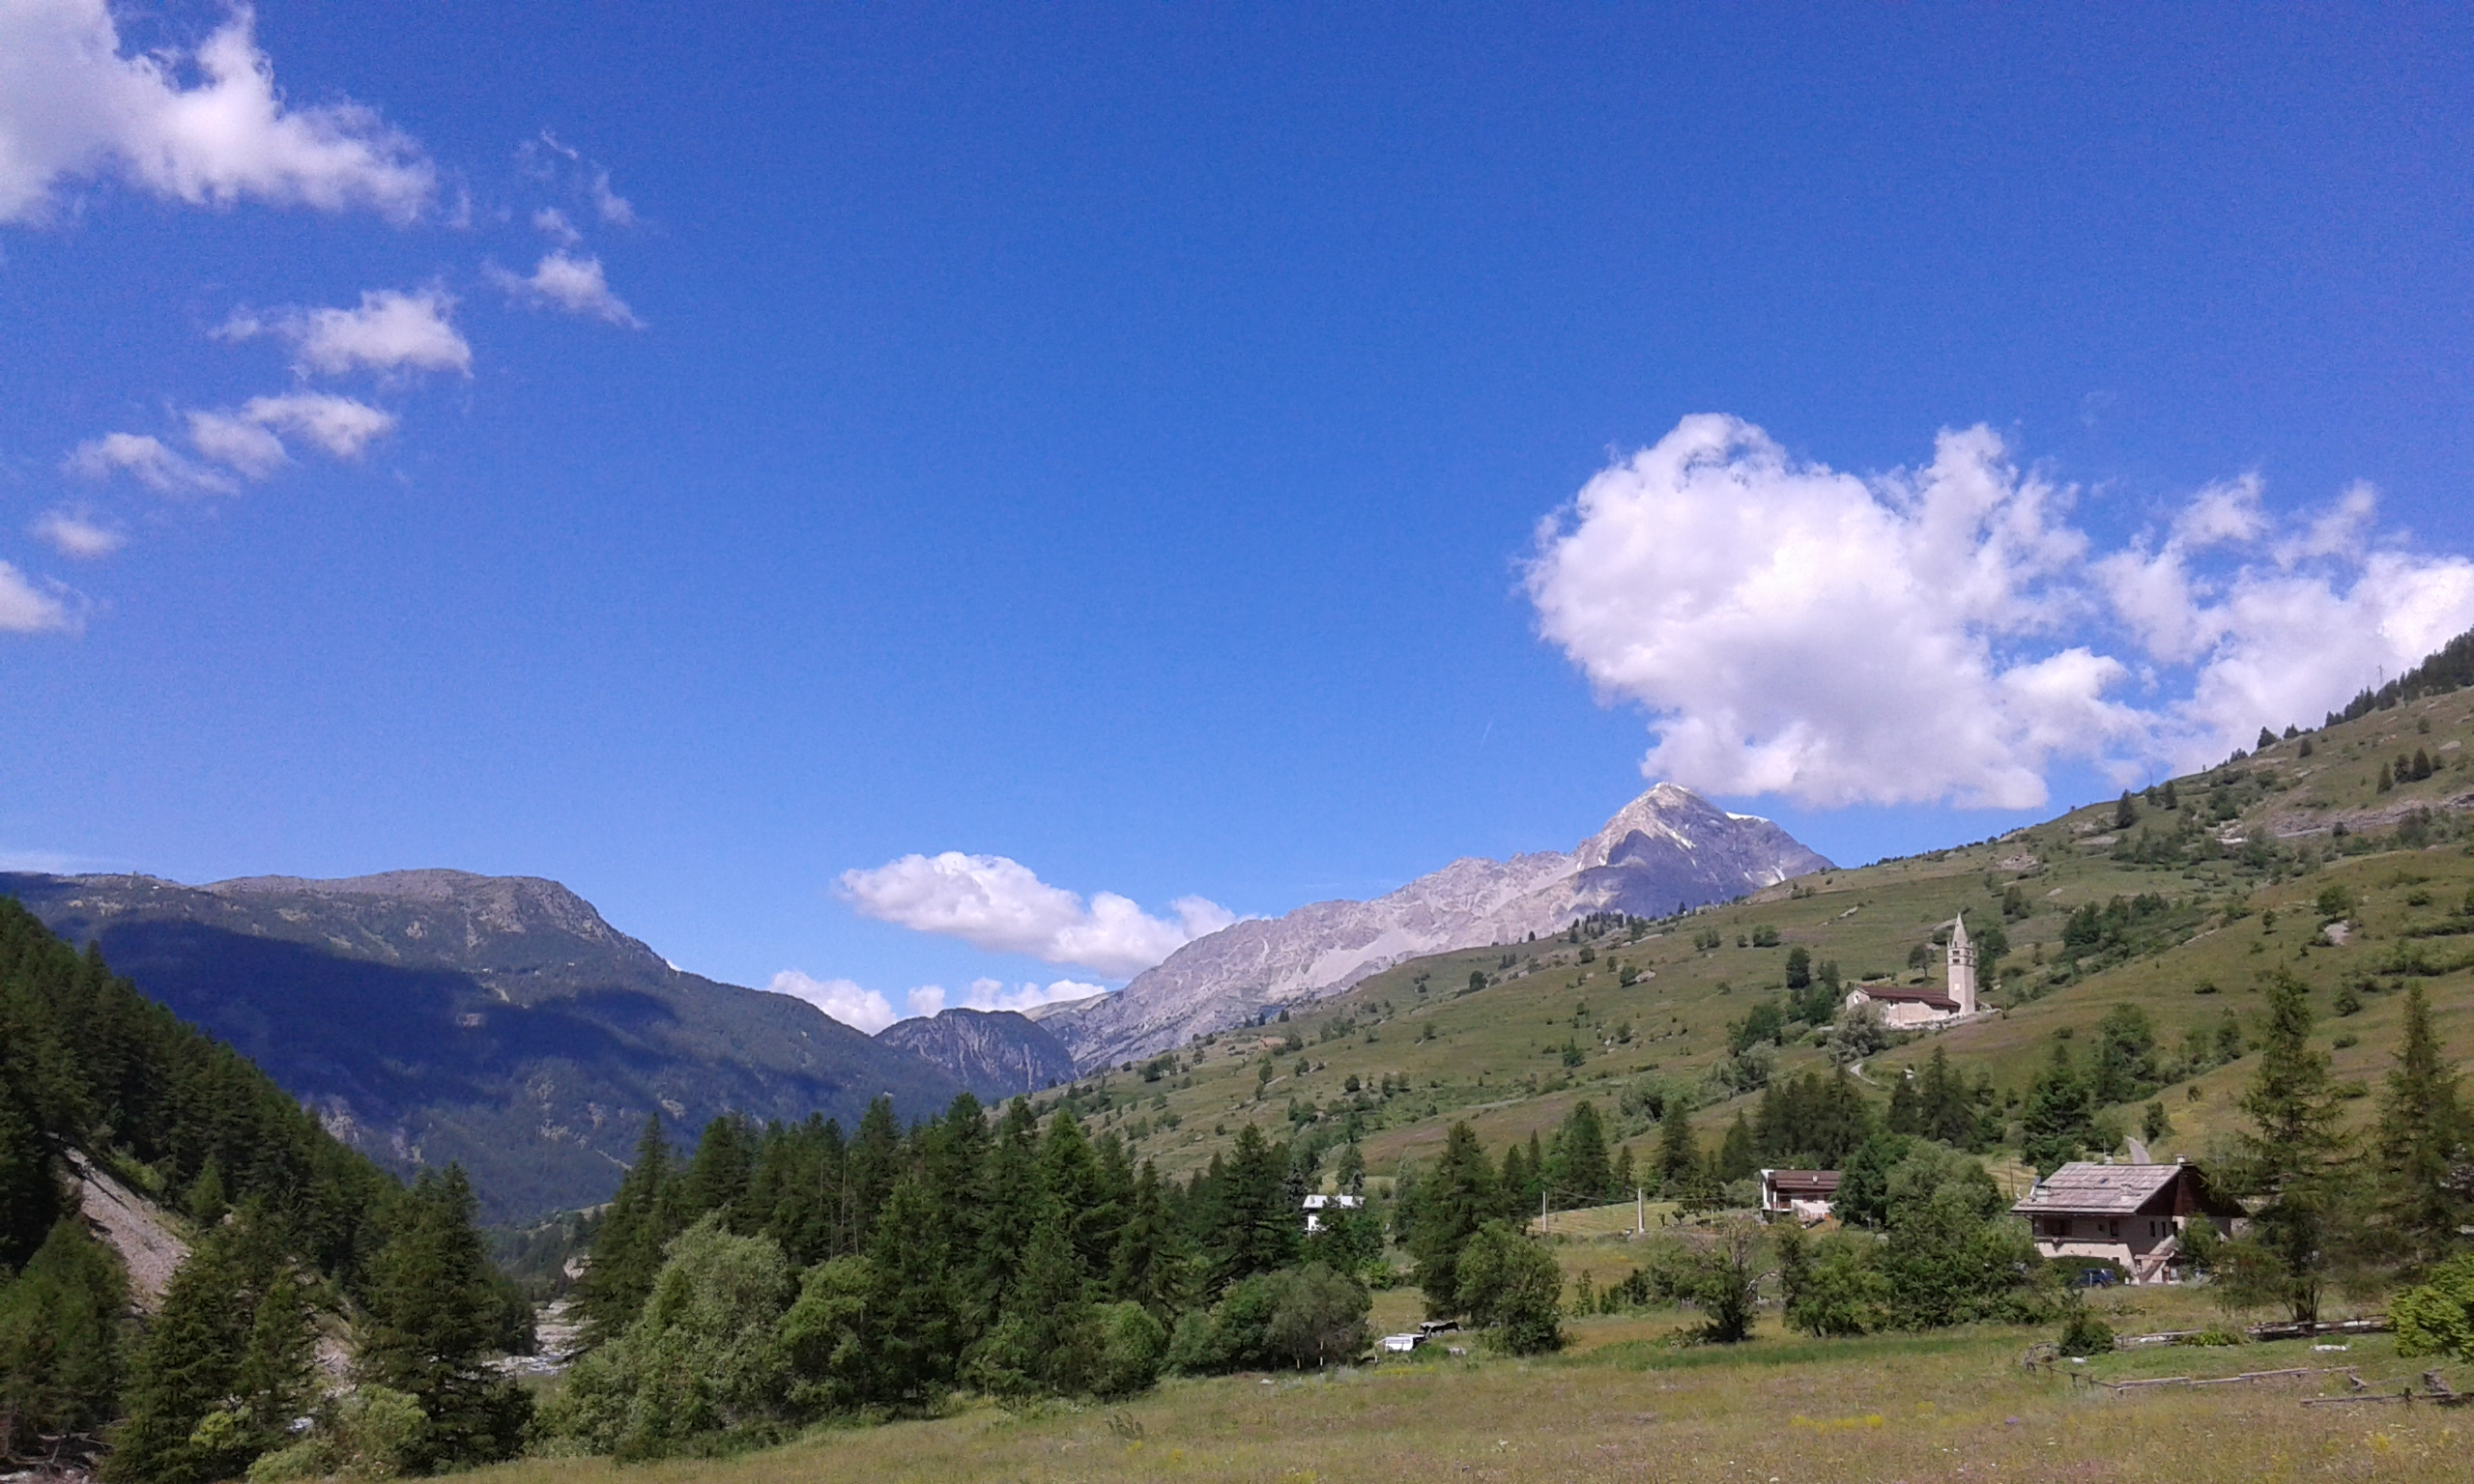
\includegraphics[width=0.9\linewidth]{images/san-restituto} \end{center}

This document was written in with the \texttt{R} package \texttt{bookdown} \citep{R-bookdown}, \citep{bookdown2016} and is under continuous development, please report any issues to \texttt{vittorio.perduca\ at\ u-paris.fr}. This work is licensed under \href{https://creativecommons.org/licenses/by-nc/4.0/}{CC BY-NC 4.0}.

\hypertarget{introduction}{%
\chapter{Introduction}\label{introduction}}

\texttt{R} is a statistical language developed from the 1990s at the University of Auckland, New Zealand. Its main implementation is the open source software (free and modifiable) \texttt{R}. \texttt{R} is normally used from the graphical user interface (GUI) and development interface RStudio.

\texttt{R} is an \href{http://www.france-ioi.org/algo/course.php?idChapter=561\&idCourse=2368}{interpreted language} (like\texttt{Python}) that we use from the command line:

\begin{Shaded}
\begin{Highlighting}[]
\KeywordTok{print}\NormalTok{ (}\StringTok{'Hello world!'}\NormalTok{)}
\end{Highlighting}
\end{Shaded}

\begin{verbatim}
## [1] "Hello world!"
\end{verbatim}

Alternatively, you can run a script, that is a series of commands found in a file with the extension \texttt{.R}.

The \texttt{R} user community is very active in the scientific world (statistics, data science, bioinformatics, social sciences, \ldots{}) and more and more in companies. One of the advantages of \texttt{R} is the wealth of \emph{packages} developed by users and developers that can be installed to increase its capabilities in many areas of statistics.

In addition, \texttt{R} has a very complete documentation. You can access help by typing \texttt{?} followed by the \emph{function} you are interested in:

\begin{Shaded}
\begin{Highlighting}[]
\NormalTok{? rnorm}
\end{Highlighting}
\end{Shaded}

You can also find a lot of information on the web: by searching on Google for a problem related to an \texttt{R} task, you almost always find an answer (often in threads opened on \href{https:\%20//\%20stats\%20.stackexchange.com\%20/}{Cross Validated}).

\hypertarget{how-to-use-this-document}{%
\section{How to use this document}\label{how-to-use-this-document}}

Although basic objects and commands are covered, this introduction is not a complete reference to the \texttt{R} language, so you will have to use the help and search for information on the web. Before moving on to the exercises at the end of each chapter, you are encouraged to type the commands and understand the result: the best way to learn a language is to write and debug lots of lines of code!

\hypertarget{useful-references}{%
\section{Useful references}\label{useful-references}}

A complete reference to \texttt{R} is the official introduction that can be found on the CRAN website: \url{https://cran.r-project.org/doc/manuals/R-intro.html}. For French readers, an excellent reference is Vincent Goulet's book \emph{Introduction à la programmation R}, which can be downloaded at \url{https://cran.r-project.org/doc/contrib/Goulet_introduction_programmation_R.pdf}

\hypertarget{installing-r-and-rstudio}{%
\section{Installing R and Rstudio}\label{installing-r-and-rstudio}}

\begin{enumerate}
\def\labelenumi{\arabic{enumi}.}
\tightlist
\item
  Download the \texttt{R} distribution that is appropriate for your machine from \url{https://cran.r-project.org/} and install it by double-clicking on the installation file.
\item
  Dowanload and install RStudio Desktop from \url{https://rstudio.com/products/rstudio/download/}.
\end{enumerate}

\hypertarget{getting-started-with-rstudio}{%
\section{Getting started with RStudio}\label{getting-started-with-rstudio}}

The RStudio workspace is generally divided into four pans: starting from the top left and going clockwise we find:

\begin{enumerate}
\def\labelenumi{\arabic{enumi}.}
\tightlist
\item
  a script editor
\item
  the environment listing the variables in memory and the history of commands that were executed
\item
  a window for graphical outputs, the help, and the file and package managers.
\item
  the \texttt{R} console, ie the command line.
\end{enumerate}

Typically we type the code in the editor and then run it in the console. To do this we place the cursor in the line we want to execute and we send the command to the console using the combination \texttt{cmd\ Return} in macOS and\texttt{ctrl\ Return} under Linux and Windows.

\hypertarget{packages}{%
\section{Packages}\label{packages}}

To install a package from the console:

\begin{Shaded}
\begin{Highlighting}[]
\KeywordTok{install.packages}\NormalTok{(}\StringTok{"dplyr"}\NormalTok{)}
\CommentTok{# download and install the dplyr package used for data manipulation}
\end{Highlighting}
\end{Shaded}

Once a package is installed, it will have to be loaded into memory each time a new session is opened:

\begin{Shaded}
\begin{Highlighting}[]
\KeywordTok{library}\NormalTok{(dplyr) }\CommentTok{# quotes are not needed here}
\CommentTok{# require(dplyr) # equivalent function}
\end{Highlighting}
\end{Shaded}

\hypertarget{language-basics}{%
\chapter{Language basics}\label{language-basics}}

\hypertarget{assignments-arithmetic-operations}{%
\section{Assignments, arithmetic operations}\label{assignments-arithmetic-operations}}

There are two types of \texttt{R} commands: expressions and assignments.

\textbf{Expression}

\begin{Shaded}
\begin{Highlighting}[]
\KeywordTok{cos}\NormalTok{(pi)}
\end{Highlighting}
\end{Shaded}

\begin{verbatim}
## [1] -1
\end{verbatim}

\textbf{Assignments and expressions}

\begin{Shaded}
\begin{Highlighting}[]
\NormalTok{x <-}\StringTok{ }\DecValTok{1} \OperatorTok{+}\StringTok{ }\DecValTok{2} \CommentTok{# or x = 1 + 2}
\NormalTok{x}
\end{Highlighting}
\end{Shaded}

\begin{verbatim}
## [1] 3
\end{verbatim}

\begin{Shaded}
\begin{Highlighting}[]
\NormalTok{y =}\StringTok{ }\DecValTok{4}
\NormalTok{x }\OperatorTok{==}\StringTok{ }\NormalTok{y}
\end{Highlighting}
\end{Shaded}

\begin{verbatim}
## [1] FALSE
\end{verbatim}

Using \texttt{;} we can type two commands on the same line before executing them:

\begin{Shaded}
\begin{Highlighting}[]
\NormalTok{e <-}\StringTok{ }\KeywordTok{exp}\NormalTok{ (}\DecValTok{1}\NormalTok{); }\KeywordTok{log}\NormalTok{ (e)}
\end{Highlighting}
\end{Shaded}

\begin{verbatim}
## [1] 1
\end{verbatim}

Some examples of arithmetic and Boolean operators:

\begin{Shaded}
\begin{Highlighting}[]
\DecValTok{3}\OperatorTok{*}\DecValTok{4}
\end{Highlighting}
\end{Shaded}

\begin{verbatim}
## [1] 12
\end{verbatim}

\begin{Shaded}
\begin{Highlighting}[]
\DecValTok{12}\OperatorTok{/}\DecValTok{3}
\end{Highlighting}
\end{Shaded}

\begin{verbatim}
## [1] 4
\end{verbatim}

\begin{Shaded}
\begin{Highlighting}[]
\DecValTok{2}\OperatorTok{^}\DecValTok{3}
\end{Highlighting}
\end{Shaded}

\begin{verbatim}
## [1] 8
\end{verbatim}

\begin{Shaded}
\begin{Highlighting}[]
\KeywordTok{sqrt}\NormalTok{ (}\DecValTok{16}\NormalTok{)}
\end{Highlighting}
\end{Shaded}

\begin{verbatim}
## [1] 4
\end{verbatim}

\begin{Shaded}
\begin{Highlighting}[]
\DecValTok{1} \OperatorTok{==}\StringTok{ }\DecValTok{2}
\end{Highlighting}
\end{Shaded}

\begin{verbatim}
## [1] FALSE
\end{verbatim}

\begin{Shaded}
\begin{Highlighting}[]
\DecValTok{1}\OperatorTok{!=}\StringTok{ }\DecValTok{1}
\end{Highlighting}
\end{Shaded}

\begin{verbatim}
## [1] FALSE
\end{verbatim}

\begin{Shaded}
\begin{Highlighting}[]
\OtherTok{FALSE} \OperatorTok{&}\StringTok{ }\OtherTok{TRUE} \CommentTok{# and}
\end{Highlighting}
\end{Shaded}

\begin{verbatim}
## [1] FALSE
\end{verbatim}

\begin{Shaded}
\begin{Highlighting}[]
\OtherTok{FALSE} \OperatorTok{|}\StringTok{ }\OtherTok{TRUE} \CommentTok{# or}
\end{Highlighting}
\end{Shaded}

\begin{verbatim}
## [1] TRUE
\end{verbatim}

\hypertarget{mode-length-and-class}{%
\section{Mode, length and class}\label{mode-length-and-class}}

In R, everything is an \emph{object}. The \emph{mode} specifies what an object can contain. The main modes are:

\begin{itemize}
\tightlist
\item
  \texttt{numeric}: real numbers
\item
  \texttt{character}: character strings
\item
  \texttt{logical}: logical values true / false
\item
  \texttt{list}: list, collection of objects
\item
  \texttt{function}: function
\end{itemize}

\texttt{numeric},\texttt{character}, and \texttt{logical} objects are \emph{simple} objects that can contain data of only one type. On the contrary, \texttt{list} mobjects are special objects that can contain other objects.

You can access the mode of an object with the \texttt{mode\ ()} function:

\begin{Shaded}
\begin{Highlighting}[]
\NormalTok{age =}\StringTok{ }\KeywordTok{c}\NormalTok{(}\DecValTok{33}\NormalTok{,}\DecValTok{28}\NormalTok{, }\DecValTok{33}\NormalTok{) }\CommentTok{# The concatenation function c() allows to create vectors}
\KeywordTok{mode}\NormalTok{(age)}
\end{Highlighting}
\end{Shaded}

\begin{verbatim}
## [1] "numeric"
\end{verbatim}

\begin{Shaded}
\begin{Highlighting}[]
\NormalTok{names <-}\StringTok{ }\KeywordTok{c}\NormalTok{(}\StringTok{'Daniel'}\NormalTok{, }\StringTok{'Jehanne'}\NormalTok{, }\StringTok{'Romain'}\NormalTok{)}
\KeywordTok{mode}\NormalTok{(names)}
\end{Highlighting}
\end{Shaded}

\begin{verbatim}
## [1] "character"
\end{verbatim}

\begin{Shaded}
\begin{Highlighting}[]
\NormalTok{my.list <-}\StringTok{ }\KeywordTok{list}\NormalTok{(}\DataTypeTok{Names =}\NormalTok{ names, }\DataTypeTok{Age =}\NormalTok{ age)}
\KeywordTok{mode}\NormalTok{(my.list)}
\end{Highlighting}
\end{Shaded}

\begin{verbatim}
## [1] "list"
\end{verbatim}

\begin{Shaded}
\begin{Highlighting}[]
\KeywordTok{mode}\NormalTok{(}\KeywordTok{is.integer}\NormalTok{(pi))}
\end{Highlighting}
\end{Shaded}

\begin{verbatim}
## [1] "logical"
\end{verbatim}

\begin{Shaded}
\begin{Highlighting}[]
\NormalTok{mode}
\end{Highlighting}
\end{Shaded}

\begin{verbatim}
## function (x) 
## {
##     if (is.expression(x)) 
##         return("expression")
##     if (is.call(x)) 
##         return(switch(deparse(x[[1L]])[1L], `(` = "(", "call"))
##     if (is.name(x)) 
##         "name"
##     else switch(tx <- typeof(x), double = , integer = "numeric", 
##         closure = , builtin = , special = "function", tx)
## }
## <bytecode: 0x7fbafcc4a5b0>
## <environment: namespace:base>
\end{verbatim}

Besides the mode, an object also has a \emph{length}, defined as the number of elements it contains:

\begin{Shaded}
\begin{Highlighting}[]
\KeywordTok{length}\NormalTok{(age)}
\end{Highlighting}
\end{Shaded}

\begin{verbatim}
## [1] 3
\end{verbatim}

\begin{Shaded}
\begin{Highlighting}[]
\KeywordTok{length}\NormalTok{(names)}
\end{Highlighting}
\end{Shaded}

\begin{verbatim}
## [1] 3
\end{verbatim}

\begin{Shaded}
\begin{Highlighting}[]
\KeywordTok{length}\NormalTok{(my.list)}
\end{Highlighting}
\end{Shaded}

\begin{verbatim}
## [1] 2
\end{verbatim}

The \emph{class} of an object specifies its behavior and therefore its way of interacting with operations and functions. An important example are \emph{data frames}: special lists whose elements all have the same length. The class of a data frame is different from that of generic lists and data frames have an indexing system that does not exist for other lists:

\begin{Shaded}
\begin{Highlighting}[]
\KeywordTok{class}\NormalTok{(my.list)}
\end{Highlighting}
\end{Shaded}

\begin{verbatim}
## [1] "list"
\end{verbatim}

\begin{Shaded}
\begin{Highlighting}[]
\NormalTok{my.data.frame =}\StringTok{ }\KeywordTok{data.frame}\NormalTok{(names, age)}
\KeywordTok{mode}\NormalTok{(my.data.frame)}
\end{Highlighting}
\end{Shaded}

\begin{verbatim}
## [1] "list"
\end{verbatim}

\begin{Shaded}
\begin{Highlighting}[]
\KeywordTok{class}\NormalTok{(my.data.frame)}
\end{Highlighting}
\end{Shaded}

\begin{verbatim}
## [1] "data.frame"
\end{verbatim}

\begin{Shaded}
\begin{Highlighting}[]
\NormalTok{my.data.frame[}\DecValTok{1}\NormalTok{,}\DecValTok{2}\NormalTok{] }\CommentTok{# to extract the 1st element from the 2nd "column"}
\end{Highlighting}
\end{Shaded}

\begin{verbatim}
## [1] 33
\end{verbatim}

\begin{Shaded}
\begin{Highlighting}[]
\CommentTok{# Try the following command:}
\CommentTok{# my.list[1,2]}
\end{Highlighting}
\end{Shaded}

A special object is the missing value \texttt{NA}. By default, its mode is \texttt{logical}, however\texttt{NA} is neither \texttt{TRUE} nor\texttt{FALSE}. To test if a value is missing we will use the \texttt{is.na\ ()} function:

\begin{Shaded}
\begin{Highlighting}[]
\OtherTok{NA} \OperatorTok{==}\StringTok{ }\OtherTok{NA} \CommentTok{# not what we want}
\end{Highlighting}
\end{Shaded}

\begin{verbatim}
## [1] NA
\end{verbatim}

\begin{Shaded}
\begin{Highlighting}[]
\KeywordTok{is.na}\NormalTok{(}\OtherTok{NA}\NormalTok{)}
\end{Highlighting}
\end{Shaded}

\begin{verbatim}
## [1] TRUE
\end{verbatim}

\begin{Shaded}
\begin{Highlighting}[]
\KeywordTok{is.na}\NormalTok{(}\KeywordTok{mean}\NormalTok{(}\KeywordTok{c}\NormalTok{(}\DecValTok{1}\NormalTok{,}\DecValTok{4}\NormalTok{, }\OtherTok{NA}\NormalTok{)))}
\end{Highlighting}
\end{Shaded}

\begin{verbatim}
## [1] TRUE
\end{verbatim}

\hypertarget{vectors-matrices-and-functions}{%
\chapter{Vectors, matrices and functions}\label{vectors-matrices-and-functions}}

\hypertarget{vectors}{%
\section{Vectors}\label{vectors}}

The \texttt{R} basic object is the \emph{vector} (a scalar is considered as a vector of length one). The most used function to create a vector is the concatenation:

\begin{Shaded}
\begin{Highlighting}[]
\NormalTok{price <-}\StringTok{ }\KeywordTok{c}\NormalTok{(}\DecValTok{150}\NormalTok{, }\DecValTok{162}\NormalTok{, }\DecValTok{155}\NormalTok{, }\DecValTok{157}\NormalTok{); price}
\end{Highlighting}
\end{Shaded}

\begin{verbatim}
## [1] 150 162 155 157
\end{verbatim}

\textbf{Indexing} is done through brackets:

\begin{Shaded}
\begin{Highlighting}[]
\NormalTok{price[}\DecValTok{1}\NormalTok{] }\CommentTok{# Unlike in Python, the first index is always 1!!}
\end{Highlighting}
\end{Shaded}

\begin{verbatim}
## [1] 150
\end{verbatim}

\begin{Shaded}
\begin{Highlighting}[]
\NormalTok{price[}\KeywordTok{c}\NormalTok{(}\FloatTok{1.3}\NormalTok{)]}
\end{Highlighting}
\end{Shaded}

\begin{verbatim}
## [1] 150
\end{verbatim}

\begin{Shaded}
\begin{Highlighting}[]
\NormalTok{price[}\OperatorTok{-}\NormalTok{(}\DecValTok{1}\OperatorTok{:}\DecValTok{2}\NormalTok{)] }\CommentTok{# to extract all elements except the 1st and 2nd}
\end{Highlighting}
\end{Shaded}

\begin{verbatim}
## [1] 155 157
\end{verbatim}

One can also use a boolean indexing vector, the extracted elements are obviously those corresponding to the \texttt{TRUE} values. For example to extract prices greater than 156:

\begin{Shaded}
\begin{Highlighting}[]
\NormalTok{price }\OperatorTok{>}\StringTok{ }\DecValTok{156} \CommentTok{# the boolean vector}
\end{Highlighting}
\end{Shaded}

\begin{verbatim}
## [1] FALSE  TRUE FALSE  TRUE
\end{verbatim}

\begin{Shaded}
\begin{Highlighting}[]
\NormalTok{price[price }\OperatorTok{>}\StringTok{ }\DecValTok{156}\NormalTok{]}
\end{Highlighting}
\end{Shaded}

\begin{verbatim}
## [1] 162 157
\end{verbatim}

An alternative is given by the \texttt{which\ ()} function which returns the indices whose elements satisfy a logical condition:

\begin{Shaded}
\begin{Highlighting}[]
\KeywordTok{which}\NormalTok{(price }\OperatorTok{>}\StringTok{ }\DecValTok{155}\NormalTok{)}
\end{Highlighting}
\end{Shaded}

\begin{verbatim}
## [1] 2 4
\end{verbatim}

\begin{Shaded}
\begin{Highlighting}[]
\NormalTok{price[}\KeywordTok{which}\NormalTok{(price }\OperatorTok{>}\StringTok{ }\DecValTok{156}\NormalTok{)]}
\end{Highlighting}
\end{Shaded}

\begin{verbatim}
## [1] 162 157
\end{verbatim}

You can use the indexing to change an element:

\begin{Shaded}
\begin{Highlighting}[]
\NormalTok{price [}\DecValTok{1}\NormalTok{] <-}\StringTok{ }\DecValTok{0}\NormalTok{; price}
\end{Highlighting}
\end{Shaded}

\begin{verbatim}
## [1]   0 162 155 157
\end{verbatim}

It is possible to give labels to the elements of a vector and extract elements based on them:

\begin{Shaded}
\begin{Highlighting}[]
\KeywordTok{names}\NormalTok{(price) }
\end{Highlighting}
\end{Shaded}

\begin{verbatim}
## NULL
\end{verbatim}

\begin{Shaded}
\begin{Highlighting}[]
\CommentTok{# NULL is a special object with NULL mode that reads "no container"}
\KeywordTok{names}\NormalTok{(price) <-}\StringTok{ }\KeywordTok{c}\NormalTok{(}\StringTok{'model.1'}\NormalTok{, }\StringTok{'model.2'}\NormalTok{, }\StringTok{'model.3'}\NormalTok{, }\StringTok{'model.4'}\NormalTok{)}
\NormalTok{price}
\end{Highlighting}
\end{Shaded}

\begin{verbatim}
## model.1 model.2 model.3 model.4 
##       0     162     155     157
\end{verbatim}

\begin{Shaded}
\begin{Highlighting}[]
\NormalTok{price[}\StringTok{'model.3'}\NormalTok{]}
\end{Highlighting}
\end{Shaded}

\begin{verbatim}
## model.3 
##     155
\end{verbatim}

In a vector, all the elements must have the same mode:

\begin{Shaded}
\begin{Highlighting}[]
\NormalTok{x <-}\StringTok{ }\KeywordTok{c}\NormalTok{(}\DecValTok{1}\NormalTok{,}\DecValTok{2}\NormalTok{, }\StringTok{'a'}\NormalTok{, }\StringTok{'b'}\NormalTok{); x}
\end{Highlighting}
\end{Shaded}

\begin{verbatim}
## [1] "1" "2" "a" "b"
\end{verbatim}

\begin{Shaded}
\begin{Highlighting}[]
\KeywordTok{mode}\NormalTok{(x)}
\end{Highlighting}
\end{Shaded}

\begin{verbatim}
## [1] "character"
\end{verbatim}

To generate the vector of the first \(n\) integers we use the syntax \texttt{1:n}

\begin{Shaded}
\begin{Highlighting}[]
\DecValTok{1}\OperatorTok{:}\DecValTok{10}
\end{Highlighting}
\end{Shaded}

\begin{verbatim}
##  [1]  1  2  3  4  5  6  7  8  9 10
\end{verbatim}

\begin{Shaded}
\begin{Highlighting}[]
\DecValTok{2}\OperatorTok{:}\DecValTok{6}
\end{Highlighting}
\end{Shaded}

\begin{verbatim}
## [1] 2 3 4 5 6
\end{verbatim}

To generate more general sequences we use the \texttt{seq()} function:

\begin{Shaded}
\begin{Highlighting}[]
\KeywordTok{seq}\NormalTok{(}\DataTypeTok{from =} \DecValTok{2}\NormalTok{, }\DataTypeTok{to =} \DecValTok{20}\NormalTok{, }\DataTypeTok{by =} \DecValTok{2}\NormalTok{) }\CommentTok{# or more simply seq(2,20,2)}
\end{Highlighting}
\end{Shaded}

\begin{verbatim}
##  [1]  2  4  6  8 10 12 14 16 18 20
\end{verbatim}

We can create a vector of repeated elements with \texttt{rep()}:

\begin{Shaded}
\begin{Highlighting}[]
\KeywordTok{rep}\NormalTok{(}\DecValTok{1}\NormalTok{, }\DataTypeTok{len =} \DecValTok{3}\NormalTok{) }\CommentTok{# same thing as rep (1,3)}
\end{Highlighting}
\end{Shaded}

\begin{verbatim}
## [1] 1 1 1
\end{verbatim}

\begin{Shaded}
\begin{Highlighting}[]
\KeywordTok{rep}\NormalTok{(}\OtherTok{NA}\NormalTok{, }\DecValTok{4}\NormalTok{)}
\end{Highlighting}
\end{Shaded}

\begin{verbatim}
## [1] NA NA NA NA
\end{verbatim}

\hypertarget{matrices}{%
\section{Matrices}\label{matrices}}

A matrix is a vector with a \texttt{dim} attribute of length two. All the elements of a matrix therefore have the same mode. To create a matrix:

\begin{Shaded}
\begin{Highlighting}[]
\NormalTok{M <-}\StringTok{ }\KeywordTok{matrix}\NormalTok{(}\DecValTok{2}\OperatorTok{:}\DecValTok{7}\NormalTok{, }\DataTypeTok{nrow =} \DecValTok{2}\NormalTok{, }\DataTypeTok{ncol =} \DecValTok{3}\NormalTok{); M}
\end{Highlighting}
\end{Shaded}

\begin{verbatim}
##      [,1] [,2] [,3]
## [1,]    2    4    6
## [2,]    3    5    7
\end{verbatim}

\begin{Shaded}
\begin{Highlighting}[]
\KeywordTok{matrix}\NormalTok{ (}\DecValTok{2}\OperatorTok{:}\DecValTok{7}\NormalTok{, }\DataTypeTok{nrow =} \DecValTok{2}\NormalTok{, }\DataTypeTok{ncol =} \DecValTok{3}\NormalTok{, }\DataTypeTok{byrow =} \OtherTok{TRUE}\NormalTok{)}
\end{Highlighting}
\end{Shaded}

\begin{verbatim}
##      [,1] [,2] [,3]
## [1,]    2    3    4
## [2,]    5    6    7
\end{verbatim}

By default \texttt{matrix\ ()} fills the new matrix one column after another. Indexing is done through brackets:

\begin{Shaded}
\begin{Highlighting}[]
\NormalTok{M[}\DecValTok{2}\NormalTok{,] }\CommentTok{# 2nd line}
\end{Highlighting}
\end{Shaded}

\begin{verbatim}
## [1] 3 5 7
\end{verbatim}

\begin{Shaded}
\begin{Highlighting}[]
\NormalTok{M[, }\DecValTok{3}\NormalTok{] }\CommentTok{# 3rd column}
\end{Highlighting}
\end{Shaded}

\begin{verbatim}
## [1] 6 7
\end{verbatim}

\begin{Shaded}
\begin{Highlighting}[]
\NormalTok{M[}\FloatTok{2.3}\NormalTok{]}
\end{Highlighting}
\end{Shaded}

\begin{verbatim}
## [1] 3
\end{verbatim}

\begin{Shaded}
\begin{Highlighting}[]
\NormalTok{M[}\DecValTok{3}\NormalTok{]}
\end{Highlighting}
\end{Shaded}

\begin{verbatim}
## [1] 4
\end{verbatim}

\begin{Shaded}
\begin{Highlighting}[]
\NormalTok{M[, }\DecValTok{-2}\NormalTok{] }\CommentTok{# to extract all columns except the 2nd}
\end{Highlighting}
\end{Shaded}

\begin{verbatim}
##      [,1] [,2]
## [1,]    2    6
## [2,]    3    7
\end{verbatim}

To vertically (resp. horizontally) merge two matrices we use \texttt{rbind()} (resp. \texttt{cbind()}):

\begin{Shaded}
\begin{Highlighting}[]
\KeywordTok{cbind}\NormalTok{ (M, }\OperatorTok{-}\NormalTok{M)}
\end{Highlighting}
\end{Shaded}

\begin{verbatim}
##      [,1] [,2] [,3] [,4] [,5] [,6]
## [1,]    2    4    6   -2   -4   -6
## [2,]    3    5    7   -3   -5   -7
\end{verbatim}

\begin{Shaded}
\begin{Highlighting}[]
\KeywordTok{rbind}\NormalTok{(M, }\DecValTok{2} \OperatorTok{*}\StringTok{ }\NormalTok{M)}
\end{Highlighting}
\end{Shaded}

\begin{verbatim}
##      [,1] [,2] [,3]
## [1,]    2    4    6
## [2,]    3    5    7
## [3,]    4    8   12
## [4,]    6   10   14
\end{verbatim}

\hypertarget{operations-on-numerical-vectors-and-matrices}{%
\section{Operations on numerical vectors and matrices}\label{operations-on-numerical-vectors-and-matrices}}

Element wise operations:

\begin{Shaded}
\begin{Highlighting}[]
\NormalTok{v <-}\StringTok{ }\KeywordTok{c}\NormalTok{(}\DecValTok{3}\NormalTok{,}\DecValTok{4}\NormalTok{,}\DecValTok{1}\NormalTok{,}\DecValTok{6}\NormalTok{)}
\NormalTok{v }\OperatorTok{+}\StringTok{ }\DecValTok{2}
\end{Highlighting}
\end{Shaded}

\begin{verbatim}
## [1] 5 6 3 8
\end{verbatim}

\begin{Shaded}
\begin{Highlighting}[]
\NormalTok{v }\OperatorTok{*}\StringTok{ }\DecValTok{2}
\end{Highlighting}
\end{Shaded}

\begin{verbatim}
## [1]  6  8  2 12
\end{verbatim}

\begin{Shaded}
\begin{Highlighting}[]
\NormalTok{v }\OperatorTok{*}\StringTok{ }\NormalTok{v}
\end{Highlighting}
\end{Shaded}

\begin{verbatim}
## [1]  9 16  1 36
\end{verbatim}

\begin{Shaded}
\begin{Highlighting}[]
\NormalTok{v }\OperatorTok{/}\StringTok{ }\DecValTok{2}
\end{Highlighting}
\end{Shaded}

\begin{verbatim}
## [1] 1.5 2.0 0.5 3.0
\end{verbatim}

\begin{Shaded}
\begin{Highlighting}[]
\NormalTok{v }\OperatorTok{/}\StringTok{ }\NormalTok{v}
\end{Highlighting}
\end{Shaded}

\begin{verbatim}
## [1] 1 1 1 1
\end{verbatim}

\begin{Shaded}
\begin{Highlighting}[]
\NormalTok{v }\OperatorTok{+}\StringTok{ }\NormalTok{v}\OperatorTok{^}\DecValTok{2}
\end{Highlighting}
\end{Shaded}

\begin{verbatim}
## [1] 12 20  2 42
\end{verbatim}

\begin{Shaded}
\begin{Highlighting}[]
\KeywordTok{sqrt}\NormalTok{(M)}
\end{Highlighting}
\end{Shaded}

\begin{verbatim}
##          [,1]     [,2]     [,3]
## [1,] 1.414214 2.000000 2.449490
## [2,] 1.732051 2.236068 2.645751
\end{verbatim}

\begin{Shaded}
\begin{Highlighting}[]
\NormalTok{M }\OperatorTok{*}\StringTok{ }\NormalTok{M}
\end{Highlighting}
\end{Shaded}

\begin{verbatim}
##      [,1] [,2] [,3]
## [1,]    4   16   36
## [2,]    9   25   49
\end{verbatim}

\begin{Shaded}
\begin{Highlighting}[]
\CommentTok{# Try the following command:}
\CommentTok{# M + v}
\end{Highlighting}
\end{Shaded}

Transpose, multiplication, inverse:

\begin{Shaded}
\begin{Highlighting}[]
\KeywordTok{t}\NormalTok{(M)}
\end{Highlighting}
\end{Shaded}

\begin{verbatim}
##      [,1] [,2]
## [1,]    2    3
## [2,]    4    5
## [3,]    6    7
\end{verbatim}

\begin{Shaded}
\begin{Highlighting}[]
\NormalTok{N <-}\StringTok{ }\NormalTok{M[, }\DecValTok{-3}\NormalTok{]}
\NormalTok{N }\OperatorTok\StringTok{ }\KeywordTok{diag}\NormalTok{(}\DecValTok{1}\NormalTok{,}\DecValTok{2}\NormalTok{) }\CommentTok{# row by column product matrix}
\end{Highlighting}
\end{Shaded}

\begin{verbatim}
##      [,1] [,2]
## [1,]    2    4
## [2,]    3    5
\end{verbatim}

\begin{Shaded}
\begin{Highlighting}[]
\CommentTok{# diag (1,2) builds the 2x2 diagonal matrix where all the}
\CommentTok{# diagonal elements are equal to 1, ie the 2x2 identity matrix}
\KeywordTok{solve}\NormalTok{(N)}
\end{Highlighting}
\end{Shaded}

\begin{verbatim}
##      [,1] [,2]
## [1,] -2.5    2
## [2,]  1.5   -1
\end{verbatim}

\begin{Shaded}
\begin{Highlighting}[]
\KeywordTok{solve}\NormalTok{(N) }\OperatorTok\StringTok{ }\NormalTok{N }\CommentTok{# checking if solve(N) is the inverse of N}
\end{Highlighting}
\end{Shaded}

\begin{verbatim}
##      [,1]         [,2]
## [1,]    1 1.776357e-15
## [2,]    0 1.000000e+00
\end{verbatim}

\textbf{The transpose of a vector is a row matrix: }

\begin{Shaded}
\begin{Highlighting}[]
\NormalTok{V <-}\StringTok{ }\KeywordTok{t}\NormalTok{(v)}
\KeywordTok{dim}\NormalTok{(V)}
\end{Highlighting}
\end{Shaded}

\begin{verbatim}
## [1] 1 4
\end{verbatim}

\begin{Shaded}
\begin{Highlighting}[]
\KeywordTok{t}\NormalTok{(V)}
\end{Highlighting}
\end{Shaded}

\begin{verbatim}
##      [,1]
## [1,]    3
## [2,]    4
## [3,]    1
## [4,]    6
\end{verbatim}

Pay attention to the following examples:

\begin{Shaded}
\begin{Highlighting}[]
\NormalTok{v }\OperatorTok\StringTok{ }\KeywordTok{t}\NormalTok{(v) }\CommentTok{# v is considered a column vector!}
\end{Highlighting}
\end{Shaded}

\begin{verbatim}
##      [,1] [,2] [,3] [,4]
## [1,]    9   12    3   18
## [2,]   12   16    4   24
## [3,]    3    4    1    6
## [4,]   18   24    6   36
\end{verbatim}

\begin{Shaded}
\begin{Highlighting}[]
\KeywordTok{t}\NormalTok{(v) }\OperatorTok\StringTok{ }\NormalTok{v }\CommentTok{# ditto}
\end{Highlighting}
\end{Shaded}

\begin{verbatim}
##      [,1]
## [1,]   62
\end{verbatim}

\begin{Shaded}
\begin{Highlighting}[]
\KeywordTok{diag}\NormalTok{(}\DecValTok{1}\NormalTok{,}\DecValTok{4}\NormalTok{) }\OperatorTok\StringTok{ }\NormalTok{v }\CommentTok{# ditto}
\end{Highlighting}
\end{Shaded}

\begin{verbatim}
##      [,1]
## [1,]    3
## [2,]    4
## [3,]    1
## [4,]    6
\end{verbatim}

\begin{Shaded}
\begin{Highlighting}[]
\NormalTok{v }\OperatorTok\StringTok{ }\NormalTok{v }\CommentTok{# v is both considered a row-vector and a column-vector}
\end{Highlighting}
\end{Shaded}

\begin{verbatim}
##      [,1]
## [1,]   62
\end{verbatim}

\hypertarget{factors}{%
\section{Factors}\label{factors}}

A factor is a vector used to represent qualitative variables, ie a variable with discrete values. Its values, or categories, are called the \texttt{levels} in \texttt{R}.

\begin{Shaded}
\begin{Highlighting}[]
\NormalTok{city <-}\StringTok{ }\KeywordTok{c}\NormalTok{(}\StringTok{'paris'}\NormalTok{, }\StringTok{'lyon'}\NormalTok{, }\StringTok{'lyon'}\NormalTok{, }\StringTok{'paris'}\NormalTok{, }\StringTok{'nantes'}\NormalTok{)}
\NormalTok{fact.city <-}\StringTok{ }\KeywordTok{as.factor}\NormalTok{(city); fact.city}
\end{Highlighting}
\end{Shaded}

\begin{verbatim}
## [1] paris  lyon   lyon   paris  nantes
## Levels: lyon nantes paris
\end{verbatim}

\begin{Shaded}
\begin{Highlighting}[]
\KeywordTok{class}\NormalTok{(fact.city)}
\end{Highlighting}
\end{Shaded}

\begin{verbatim}
## [1] "factor"
\end{verbatim}

\begin{Shaded}
\begin{Highlighting}[]
\KeywordTok{levels}\NormalTok{(fact.city)}
\end{Highlighting}
\end{Shaded}

\begin{verbatim}
## [1] "lyon"   "nantes" "paris"
\end{verbatim}

A factor has the \texttt{numeric} mode. The reason for this counter-intuitive fact is that the elements of a factor are represented as integers corresponding to the lexicographic order of their values:

\begin{Shaded}
\begin{Highlighting}[]
\KeywordTok{mode}\NormalTok{(fact.city)}
\end{Highlighting}
\end{Shaded}

\begin{verbatim}
## [1] "numeric"
\end{verbatim}

\begin{Shaded}
\begin{Highlighting}[]
\KeywordTok{as.numeric}\NormalTok{(fact.city)}
\end{Highlighting}
\end{Shaded}

\begin{verbatim}
## [1] 3 1 1 3 2
\end{verbatim}

\hypertarget{user-defined-functions}{%
\section{User-defined functions}\label{user-defined-functions}}

\textbf{Example:}

\begin{Shaded}
\begin{Highlighting}[]
\NormalTok{my.function <-}\StringTok{ }\ControlFlowTok{function}\NormalTok{(x, }\DataTypeTok{y =} \DecValTok{10}\NormalTok{) \{}\CommentTok{# the default value of y is 10}
\NormalTok{  z =}\StringTok{ }\NormalTok{x}\OperatorTok{-}\NormalTok{y}
  \KeywordTok{return}\NormalTok{(z)}
\NormalTok{\}}
\KeywordTok{my.function}\NormalTok{(}\DecValTok{2}\NormalTok{)}
\end{Highlighting}
\end{Shaded}

\begin{verbatim}
## [1] -8
\end{verbatim}

\begin{Shaded}
\begin{Highlighting}[]
\KeywordTok{my.function}\NormalTok{(}\DecValTok{2}\NormalTok{,}\DecValTok{4}\NormalTok{)}
\end{Highlighting}
\end{Shaded}

\begin{verbatim}
## [1] -2
\end{verbatim}

\begin{Shaded}
\begin{Highlighting}[]
\KeywordTok{my.function}\NormalTok{(}\DataTypeTok{y =} \DecValTok{1}\NormalTok{, }\DataTypeTok{x =} \DecValTok{4}\NormalTok{)}
\end{Highlighting}
\end{Shaded}

\begin{verbatim}
## [1] 3
\end{verbatim}

Any variable defined in a function is \emph{local} and does not appear in the workspace: try to run

\begin{Shaded}
\begin{Highlighting}[]
\NormalTok{z}
\end{Highlighting}
\end{Shaded}

\hypertarget{lists-and-data-frames}{%
\chapter{Lists and data frames}\label{lists-and-data-frames}}

\hypertarget{lists}{%
\section{Lists}\label{lists}}

Lists are special vectors that can store elements of any mode (including other lists).

\begin{Shaded}
\begin{Highlighting}[]
\NormalTok{age =}\StringTok{ }\KeywordTok{c}\NormalTok{(}\DecValTok{33}\NormalTok{,}\DecValTok{28}\NormalTok{, }\DecValTok{33}\NormalTok{)}
\NormalTok{names <-}\StringTok{ }\KeywordTok{c}\NormalTok{(}\StringTok{'Daniel'}\NormalTok{, }\StringTok{'Jehanne'}\NormalTok{, }\StringTok{'Romain'}\NormalTok{)}
\NormalTok{my.list <-}\StringTok{ }\KeywordTok{list}\NormalTok{(}\DataTypeTok{Names =}\NormalTok{ names, }\DataTypeTok{Age =}\NormalTok{ age)}
\end{Highlighting}
\end{Shaded}

Like any other vector, a list is indexed by the \texttt{{[}...{]}} operator, however, note that the result will be a list containing as unique element the desired item:

\begin{Shaded}
\begin{Highlighting}[]
\NormalTok{my.list[}\DecValTok{1}\NormalTok{]}
\end{Highlighting}
\end{Shaded}

\begin{verbatim}
## $Names
## [1] "Daniel"  "Jehanne" "Romain"
\end{verbatim}

\begin{Shaded}
\begin{Highlighting}[]
\KeywordTok{mode}\NormalTok{(my.list[}\DecValTok{1}\NormalTok{])}
\end{Highlighting}
\end{Shaded}

\begin{verbatim}
## [1] "list"
\end{verbatim}

To get the desired item directly, we therefore use the \texttt{{[}{[}...{]}{]}} operator or the \texttt{\$} operator followed by the name of the element (if available):

\begin{Shaded}
\begin{Highlighting}[]
\NormalTok{my.list[[}\DecValTok{1}\NormalTok{]]}
\end{Highlighting}
\end{Shaded}

\begin{verbatim}
## [1] "Daniel"  "Jehanne" "Romain"
\end{verbatim}

\begin{Shaded}
\begin{Highlighting}[]
\NormalTok{my.list}\OperatorTok{$}\NormalTok{age}
\end{Highlighting}
\end{Shaded}

\begin{verbatim}
## NULL
\end{verbatim}

The elements of a list can have different lengths:

\begin{Shaded}
\begin{Highlighting}[]
\NormalTok{city <-}\StringTok{ }\KeywordTok{c}\NormalTok{(}\StringTok{'paris'}\NormalTok{, }\StringTok{'lyon'}\NormalTok{, }\StringTok{'lyon'}\NormalTok{, }\StringTok{'paris'}\NormalTok{, }\StringTok{'nantes'}\NormalTok{)}
\NormalTok{my.list}\OperatorTok{$}\NormalTok{city <-}\StringTok{ }\NormalTok{city}
\NormalTok{my.list}
\end{Highlighting}
\end{Shaded}

\begin{verbatim}
## $Names
## [1] "Daniel"  "Jehanne" "Romain" 
## 
## $Age
## [1] 33 28 33
## 
## $city
## [1] "paris"  "lyon"   "lyon"   "paris"  "nantes"
\end{verbatim}

\hypertarget{data-frames}{%
\section{Data frames}\label{data-frames}}

The most widely data containers is the data frame, a special list of class \texttt{data.frame} in which all elements have the same length. For this reason, a data frame is represented in the form of a two-dimensional array whose columns are its elements. Typically, in a data frame the columns represent the \textbf{variables} and the rows the \textbf{observations}. Unlike matrices, the elements of a data frame can have different modes.

\begin{Shaded}
\begin{Highlighting}[]
\NormalTok{id <-}\StringTok{ }\KeywordTok{c}\NormalTok{(}\StringTok{'id.453'}\NormalTok{, }\StringTok{'id.452'}\NormalTok{, }\StringTok{'id.455'}\NormalTok{, }\StringTok{'id.459'}\NormalTok{, }\StringTok{'id.458'}\NormalTok{, }\StringTok{'id.456'}\NormalTok{, }\StringTok{'id.450'}\NormalTok{, }\StringTok{'id. 451'}\NormalTok{)}
\NormalTok{age <-}\StringTok{ }\KeywordTok{c}\NormalTok{ (}\DecValTok{19}\NormalTok{, }\DecValTok{45}\NormalTok{, }\DecValTok{67}\NormalTok{, }\DecValTok{53}\NormalTok{, }\DecValTok{17}\NormalTok{, }\DecValTok{30}\NormalTok{, }\DecValTok{27}\NormalTok{, }\DecValTok{35}\NormalTok{)}
\NormalTok{smoker <-}\StringTok{ }\KeywordTok{c}\NormalTok{ (}\OtherTok{TRUE}\NormalTok{, }\OtherTok{FALSE}\NormalTok{, }\OtherTok{TRUE}\NormalTok{, }\OtherTok{TRUE}\NormalTok{, }\OtherTok{FALSE}\NormalTok{, }\OtherTok{TRUE}\NormalTok{, }\OtherTok{TRUE}\NormalTok{, }\OtherTok{TRUE}\NormalTok{)}
\NormalTok{sex <-}\StringTok{ }\KeywordTok{c}\NormalTok{ (}\StringTok{'f'}\NormalTok{, }\StringTok{'f'}\NormalTok{, }\StringTok{'h'}\NormalTok{, }\StringTok{'h'}\NormalTok{, }\StringTok{'f'}\NormalTok{, }\StringTok{'h'}\NormalTok{, }\StringTok{'f'}\NormalTok{, }\StringTok{'f'}\NormalTok{)}
\NormalTok{my.db <-}\StringTok{ }\KeywordTok{data.frame}\NormalTok{ (}\DataTypeTok{Id =}\NormalTok{ id, }\DataTypeTok{Age =}\NormalTok{ age, }\DataTypeTok{Smoker =}\NormalTok{ smoker, }\DataTypeTok{Sex =}\NormalTok{ sex); my.db}
\end{Highlighting}
\end{Shaded}

\begin{verbatim}
##        Id Age Smoker Sex
## 1  id.453  19   TRUE   f
## 2  id.452  45  FALSE   f
## 3  id.455  67   TRUE   h
## 4  id.459  53   TRUE   h
## 5  id.458  17  FALSE   f
## 6  id.456  30   TRUE   h
## 7  id.450  27   TRUE   f
## 8 id. 451  35   TRUE   f
\end{verbatim}

\begin{Shaded}
\begin{Highlighting}[]
\KeywordTok{dim}\NormalTok{(my.db); }\KeywordTok{nrow}\NormalTok{(my.db); }\KeywordTok{ncol}\NormalTok{(my.db)}
\end{Highlighting}
\end{Shaded}

\begin{verbatim}
## [1] 8 4
\end{verbatim}

\begin{verbatim}
## [1] 8
\end{verbatim}

\begin{verbatim}
## [1] 4
\end{verbatim}

\begin{Shaded}
\begin{Highlighting}[]
\KeywordTok{names}\NormalTok{(my.db)}
\end{Highlighting}
\end{Shaded}

\begin{verbatim}
## [1] "Id"     "Age"    "Smoker" "Sex"
\end{verbatim}

A data frame being a list, we can extract a column using the \texttt{\$} operator preceded by the name of the data frame and followed by the name of the column (or variable), or use the operator \texttt{{[}...{]}}

\begin{Shaded}
\begin{Highlighting}[]
\NormalTok{my.db}\OperatorTok{$}\NormalTok{Sex }\CommentTok{# a column of characters is automatically transformed into a factor}
\end{Highlighting}
\end{Shaded}

\begin{verbatim}
## [1] f f h h f h f f
## Levels: f h
\end{verbatim}

\begin{Shaded}
\begin{Highlighting}[]
\NormalTok{my.db[, }\DecValTok{2}\NormalTok{]}
\end{Highlighting}
\end{Shaded}

\begin{verbatim}
## [1] 19 45 67 53 17 30 27 35
\end{verbatim}

\begin{Shaded}
\begin{Highlighting}[]
\NormalTok{my.db}\OperatorTok{$}\NormalTok{Age[my.db}\OperatorTok{$}\NormalTok{Smoker }\OperatorTok{==}\StringTok{ }\OtherTok{FALSE}\NormalTok{] }\CommentTok{# simple example of selection}
\end{Highlighting}
\end{Shaded}

\begin{verbatim}
## [1] 45 17
\end{verbatim}

The columns are directly accessible in the workspace (without having to type the name of the data frame and the \texttt{\$}) after having \emph{attached} the data frame:

\begin{Shaded}
\begin{Highlighting}[]
\KeywordTok{attach}\NormalTok{(my.db)}
\NormalTok{Age}
\end{Highlighting}
\end{Shaded}

\begin{verbatim}
## [1] 19 45 67 53 17 30 27 35
\end{verbatim}

To display only the first six lines:

\begin{Shaded}
\begin{Highlighting}[]
\KeywordTok{head}\NormalTok{(my.db)}
\end{Highlighting}
\end{Shaded}

\begin{verbatim}
##       Id Age Smoker Sex
## 1 id.453  19   TRUE   f
## 2 id.452  45  FALSE   f
## 3 id.455  67   TRUE   h
## 4 id.459  53   TRUE   h
## 5 id.458  17  FALSE   f
## 6 id.456  30   TRUE   h
\end{verbatim}

Similarly, \texttt{tail()} creates a data frame with the last six columns.

\hypertarget{importing-and-exporting-data}{%
\section{Importing and exporting data}\label{importing-and-exporting-data}}

Importing data is a fundamental step in data analysis. To load the data stored in a file (texte, .csv, Excel, \ldots{}) into the workspace (ie into memory), you can use the basic function \texttt{read.table()}. The three most important arguments are:

\begin{itemize}
\tightlist
\item
  \texttt{file}: name (and path) of the file, in quotes
\item
  \texttt{header}: are the elements of the first row the names of the columns?
\item
  \texttt{sep}: character separating the columns
\end{itemize}

\texttt{read.table()} returns a data frame:

\begin{Shaded}
\begin{Highlighting}[]
\NormalTok{url1 <-}\StringTok{ 'https://raw.githubusercontent.com/vittorioperduca/Introduction-to-R/master/data/iris.txt'}
\NormalTok{d1 <-}\StringTok{ }\KeywordTok{read.table}\NormalTok{(url1,}
                 \CommentTok{# the first line contains the name of the variables}
                 \DataTypeTok{header =} \OtherTok{TRUE}\NormalTok{,}
                 \CommentTok{# values are separated by ;}
                 \DataTypeTok{sep =} \StringTok{';'}\NormalTok{) }

\KeywordTok{head}\NormalTok{ (d1)}
\end{Highlighting}
\end{Shaded}

\begin{verbatim}
##   Sepal.Length Sepal.Width Petal.Length Petal.Width Species
## 1          5.1         3.5          1.4         0.2  setosa
## 2          4.9         3.0          1.4         0.2  setosa
## 3          4.7         3.2          1.3         0.2  setosa
## 4          4.6         3.1          1.5         0.2  setosa
## 5          5.0         3.6          1.4         0.2  setosa
## 6          5.4         3.9          1.7         0.4  setosa
\end{verbatim}

\begin{Shaded}
\begin{Highlighting}[]
\NormalTok{url2 <-}\StringTok{ 'https://raw.githubusercontent.com/vittorioperduca/Introduction-to-R/master/data/heart.txt'}
\NormalTok{d2 <-}\StringTok{ }\KeywordTok{read.table}\NormalTok{(url2,}
                 \DataTypeTok{header =} \OtherTok{TRUE}\NormalTok{,}
                 \CommentTok{# variables are separated by a tabulation}
                 \DataTypeTok{sep =} \StringTok{'}\CharTok{\textbackslash{}t}\StringTok{'}\NormalTok{) }
\KeywordTok{dim}\NormalTok{(d2); }\KeywordTok{names}\NormalTok{(d2)}
\end{Highlighting}
\end{Shaded}

\begin{verbatim}
## [1] 270  13
\end{verbatim}

\begin{verbatim}
##  [1] "age"          "sexe"         "type_douleur" "pression"     "cholester"   
##  [6] "sucre"        "electro"      "taux_max"     "angine"       "depression"  
## [11] "pic"          "vaisseau"     "coeur"
\end{verbatim}

For data stored in the \texttt{.Rda} or \texttt{.Rdata} format, the import is done with \texttt{load()} with the argument \texttt{file\ =\ filename}. For instance download the \texttt{Iris.Rda} file at \href{https://github.com/vittorioperduca/Introduction-to-R/blob/master/data/Iris.Rda}{github.com/vittorioperduca/Introduction-to-R/blob/master/data/Iris.Rda} to your working directory and then try the following:

\begin{Shaded}
\begin{Highlighting}[]
\NormalTok{iris_path <-}\StringTok{ 'data/Iris.Rda'} \CommentTok{# replace with the file path}
\KeywordTok{load}\NormalTok{(iris_path)}
\end{Highlighting}
\end{Shaded}

If you want to load \texttt{.Rda} or \texttt{.Rdata} files directly from an url, don't forget to use the \texttt{url()} function (this was not necessary in \texttt{read.table()}).

Data can be exported either to a text file (or .csv, Excel \ldots{}) using \texttt{write.file()} or to \texttt{.rda} and \texttt{.Rdata} files at using \texttt{save()}. In both cases, the two main arguments are

\begin{itemize}
\tightlist
\item
  \texttt{x\ =} data to save
\item
  \texttt{file\ =} the name of the file (in quotes).
\end{itemize}

If the dataset is stored (or must be saved up) locally, it is necessary to know (and be able to modify) the working directory:

\begin{Shaded}
\begin{Highlighting}[]
\CommentTok{# getwd() # try on your machine!}
\CommentTok{# setwd('~/Documents') # to move to the Documents directory}
\end{Highlighting}
\end{Shaded}

Remember that in Linux and macOS machines, \texttt{\textasciitilde{}/} is a shortcut for \texttt{/Users/username}. For Windows machines, the address syntax is slightly different. For example we use \texttt{\textbackslash{}} instead of \texttt{/}.

\hypertarget{exercice}{%
\section{Exercice}\label{exercice}}

Download the text file \href{https://raw.githubusercontent.com/vittorioperduca/Introduction-to-R/master/data/hepatitis.txt}{raw.githubusercontent.com/vittorioperduca/Introduction-to-R/master/data/hepatitis.txt} to your working directory.

\begin{enumerate}
\def\labelenumi{\arabic{enumi}.}
\tightlist
\item
  Import the dataset in \texttt{R}. Warning: missing data were coded with a \texttt{?}, read the documentation of \texttt{read.table\ ()}.
\item
  Find the number of observations, display the names of the variables and the first six observations. Check that the value of \texttt{STEROID} for the fourth observation is missing using the appropriate function.
\item
  Calculate the mean value of \texttt{ALBUMIN} in women and men.
\item
  Create a variable \texttt{NSYMP} counting the number of times a variable is equal to\texttt{yes} between \texttt{FATIGUE} and\texttt{MALAISE}. Pay attention to the format of these two variables!
\end{enumerate}

\bibliography{ref.bib}

\end{document}
